\documentclass[tikz, border=10pt]{standalone}
\usetikzlibrary{positioning, calc, backgrounds, shapes.geometric}

\begin{document}
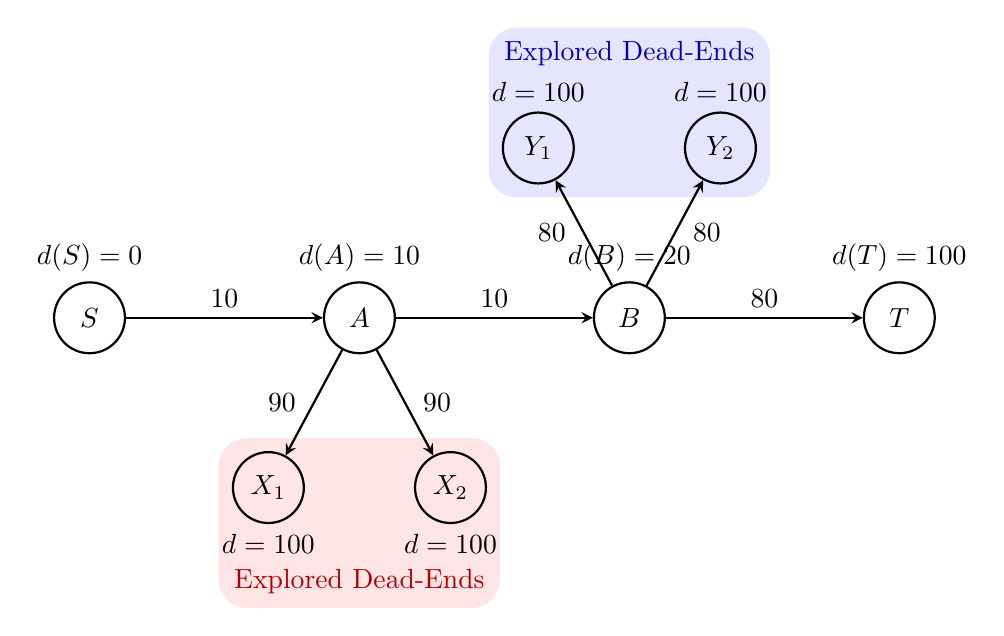
\begin{tikzpicture}[
    node distance=2cm and 2.5cm,
    vertex/.style={circle, draw, thick, minimum size=0.9cm, inner sep=1pt},
    directed/.style={->, >=stealth, thick}
]

\node[vertex, label=above:{$d(S)=0$}] (S) {$S$};
\node[vertex, right=of S, label=above:{$d(A)=10$}] (A) {$A$};
\node[vertex, right=of A, label=above:{$d(B)=20$}] (B) {$B$};
\node[vertex, right=of B, label=above:{$d(T)=100$}] (T) {$T$};

\draw[directed] (S) -- node[above] {10} (A);
\draw[directed] (A) -- node[above] {10} (B);
\draw[directed] (B) -- node[above] {80} (T);

\node[vertex, below left=1.5cm and 0.5cm of A, label=below:{$d=100$}] (X1) {$X_1$};
\node[vertex, below right=1.5cm and 0.5cm of A, label=below:{$d=100$}] (X2) {$X_2$};
\draw[directed] (A) -- node[left, xshift=-0.1cm] {90} (X1);
\draw[directed] (A) -- node[right, xshift=0.1cm] {90} (X2);

% Παγίδες (dead-ends) από τον κόμβο B
\node[vertex, above left=1.5cm and 0.5cm of B, label=above:{$d=100$}] (Y1) {$Y_1$};
\node[vertex, above right=1.5cm and 0.5cm of B, label=above:{$d=100$}] (Y2) {$Y_2$};
\draw[directed] (B) -- node[left, xshift=-0.1cm] {80} (Y1);
\draw[directed] (B) -- node[right, xshift=0.1cm] {80} (Y2);

\begin{scope}[on background layer]
    \fill[red!10, rounded corners=10pt] 
        ($(X1.south west)+(-0.3,-1.2)$) rectangle ($(X2.north east)+(0.3, 0.3)$);
    \node[red!70!black] at ($(X1)!0.5!(X2) - (0, 1.2)$) {Explored Dead-Ends};
    
    \fill[blue!10, rounded corners=10pt] 
        ($(Y1.south west)+(-0.3,-0.3)$) rectangle ($(Y2.north east)+(0.3, 1.2)$);
    \node[blue!70!black] at ($(Y1)!0.5!(Y2) + (0, 1.2)$) {Explored Dead-Ends};
\end{scope}

\end{tikzpicture}
\end{document}